\begin{pastexam}[label={px:ntut-107-ci-01}]{北科大資工所 107 學年度 第 1 題（節錄 (2)(3)(4) 小題）}
（簡答；第 (1) 小題是離散數學，未收）

(12 pts) Please answer the following questions shortly and concisely.
\begin{enumerate}[label=(\arabic*)]
\setcounter{enumi}{1}
\item (3 pts) Please convert the following expression in an infix form into a postfix form.
\[ 6+5*3-7-8+9*2 \]
\item (3 pts) Suppose that we use bottom-up heap construction to build up a \textit{minimum heap}
with an array of keys initially shown as below.
\begin{center}
\begin{tabular}{|*{15}{c|}}
\hline
16 & 24 & 8 & 15 & 4 & 30 & 11 & 33 & 7 & 40 & 27 & 18 & 42 & 22 & 3 \\ \hline
\end{tabular}
\end{center}
After the construction, what is the key value at the last position of the array?
\item (3 pts) Please give a red-black tree that is not an AVL tree and explain why.
\end{enumerate}
\end{pastexam}

\begin{pastsoln}
答案：(2) \texttt{6 5 3 * + 7 - 8 - 9 2 * +}；(3) $16$；(4) 見下面的樹。

\textbf{(2)} 用資結書虛擬碼~6.8 的堆疊做法：運算元直接輸出；遇到運算子時，先把堆疊頂端優先序
\textbf{大於或等於}它的運算子彈出（$+$、$-$ 是左結合，同級也要先彈），再把它推入；最後把堆疊
清空。
\begin{center}
\small
\begin{tabular}{clll}
\toprule
讀入 & 動作 & 堆疊（右邊是頂端） & 輸出 \\
\midrule
6 & 輸出 & & 6 \\
$+$ & 推入 & $+$ & 6 \\
5 & 輸出 & $+$ & 6 5 \\
$*$ & $*$ 比 $+$ 高，推入 & $+\;*$ & 6 5 \\
3 & 輸出 & $+\;*$ & 6 5 3 \\
$-$ & 彈出 $*$、$+$，推入 $-$ & $-$ & 6 5 3 $*$ $+$ \\
7 & 輸出 & $-$ & 6 5 3 $*$ $+$ 7 \\
$-$ & 彈出 $-$，推入 $-$ & $-$ & 6 5 3 $*$ $+$ 7 $-$ \\
8 & 輸出 & $-$ & 6 5 3 $*$ $+$ 7 $-$ 8 \\
$+$ & 彈出 $-$，推入 $+$ & $+$ & 6 5 3 $*$ $+$ 7 $-$ 8 $-$ \\
9 & 輸出 & $+$ & $\cdots$ 8 $-$ 9 \\
$*$ & $*$ 比 $+$ 高，推入 & $+\;*$ & $\cdots$ 8 $-$ 9 \\
2 & 輸出 & $+\;*$ & $\cdots$ 8 $-$ 9 2 \\
結束 & 彈出 $*$、$+$ & & $\cdots$ 8 $-$ 9 2 $*$ $+$ \\
\bottomrule
\end{tabular}
\end{center}
後序式是 \texttt{6 5 3 * + 7 - 8 - 9 2 * +}。 核對：照後序求值，$5 \cdot 3 = 15$、$6 + 15 = 21$、
$21 - 7 = 14$、$14 - 8 = 6$、$9 \cdot 2 = 18$、$6 + 18 = 24$；原式
$6 + 15 - 7 - 8 + 18 = 24$，一致。 最容易錯的是把 \texttt{7 - 8} 寫成 \texttt{7 8 -}，
那是 $7 - 8$ 先算，變成 $6 + 15 - (7 - 8)$，值不對。

\textbf{(3)} 由下而上建堆積（資結書虛擬碼~8.3，最小堆積版）：陣列從 $1$ 開始編號，$n = 15$，從最後
一個內部節點 $\lfloor 15/2 \rfloor = 7$ 往回到 $1$，每個位置做一次下沉，和\textbf{較小}的子節點交換。
\begin{center}
\small
\setlength{\tabcolsep}{3.5pt}
\begin{tabular}{l*{15}{c}}
\toprule
位置 & 1 & 2 & 3 & 4 & 5 & 6 & 7 & 8 & 9 & 10 & 11 & 12 & 13 & 14 & 15 \\
\midrule
開始 & 16 & 24 & 8 & 15 & 4 & 30 & 11 & 33 & 7 & 40 & 27 & 18 & 42 & 22 & 3 \\
$i = 7$ & 16 & 24 & 8 & 15 & 4 & 30 & \textbf{3} & 33 & 7 & 40 & 27 & 18 & 42 & 22 & \textbf{11} \\
$i = 6$ & 16 & 24 & 8 & 15 & 4 & \textbf{18} & 3 & 33 & 7 & 40 & 27 & \textbf{30} & 42 & 22 & 11 \\
$i = 5$ & 16 & 24 & 8 & 15 & 4 & 18 & 3 & 33 & 7 & 40 & 27 & 30 & 42 & 22 & 11 \\
$i = 4$ & 16 & 24 & 8 & \textbf{7} & 4 & 18 & 3 & 33 & \textbf{15} & 40 & 27 & 30 & 42 & 22 & 11 \\
$i = 3$ & 16 & 24 & \textbf{3} & 7 & 4 & 18 & \textbf{8} & 33 & 15 & 40 & 27 & 30 & 42 & 22 & 11 \\
$i = 2$ & 16 & \textbf{4} & 3 & 7 & \textbf{24} & 18 & 8 & 33 & 15 & 40 & 27 & 30 & 42 & 22 & 11 \\
$i = 1$ & \textbf{3} & 4 & \textbf{8} & 7 & 24 & 18 & \textbf{11} & 33 & 15 & 40 & 27 & 30 & 42 & 22 & \textbf{16} \\
\bottomrule
\end{tabular}
\end{center}
各步說明（粗體是這一步動到的格子）：
\begin{itemize}
\item $i = 7$：$11$ 的子節點是 $A[14] = 22$、$A[15] = 3$，和 $3$ 交換。
\item $i = 6$：$30$ 的子節點是 $18$、$42$，和 $18$ 交換。
\item $i = 5$：$4$ 比子節點 $40$、$27$ 都小，不動。
\item $i = 4$：$15$ 的子節點是 $33$、$7$，和 $7$ 交換。
\item $i = 3$：$8$ 的子節點是 $18$、$3$，和 $3$ 交換；$8$ 到了位置 $7$，子節點 $22$、$11$ 都比它大，停。
\item $i = 2$：$24$ 的子節點是 $7$、$4$，和 $4$ 交換；到了位置 $5$，子節點 $40$、$27$ 都比它大，停。
\item $i = 1$：$16$ 的子節點是 $4$、$3$，和 $3$ 交換；到位置 $3$，子節點 $18$、$8$，和 $8$ 交換；到位置
$7$，子節點 $22$、$11$，和 $11$ 交換；到位置 $15$，是葉節點，停。
\end{itemize}
最後一格 $A[15] = 16$。 注意由下而上建堆積和「一個一個插入」得到的陣列不一定相同；題目指定
bottom-up，要照下沉的做法。

\textbf{(4)} 例子（黑色實心是黑節點，紅框白底是紅節點，NIL 葉子沒畫）：
\begin{center}
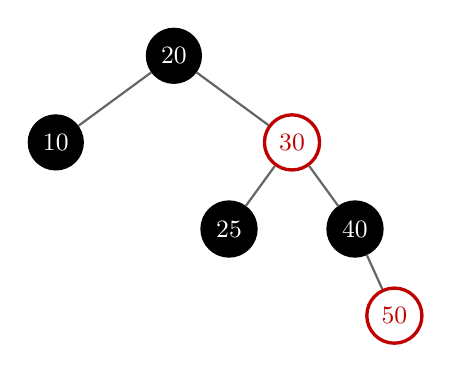
\begin{tikzpicture}[
    bk/.style={circle, draw=black, fill=black, text=white, minimum size=7mm, inner sep=0pt, font=\small},
    rd/.style={circle, draw=red!75!black, line width=1.2pt, fill=white, text=red!75!black, minimum size=7mm, inner sep=0pt, font=\small},
    level distance=11mm, edge from parent/.style={draw=black!60, thick},
    level 1/.style={sibling distance=30mm}, level 2/.style={sibling distance=16mm},
    level 3/.style={sibling distance=10mm}]
\node[bk] {20}
    child {node[bk] {10}}
    child {node[rd] {30}
        child {node[bk] {25}}
        child {node[bk] {40}
            child[missing]
            child {node[rd] {50}}}};
\end{tikzpicture}
\end{center}
\textbf{它是紅黑樹}（資結書第~10.3~節的性質）：根 $20$ 是黑的；唯一的兩個紅節點 $30$、$50$ 的子節點
（$25$、$40$ 和兩個 NIL）都是黑的，沒有紅紅相連；每個節點到它子孫 NIL 的每條路徑上，黑節點數相同。
從根算（不算 NIL）：$20 \to 10$ 有 $2$ 個黑節點；$20 \to 30 \to 25$ 是 $20$、$25$ 兩個；
$20 \to 30 \to 40$、$20 \to 30 \to 40 \to 50$ 都是 $20$、$40$ 兩個，黑高度都是 $2$。 中序是
$10, 20, 25, 30, 40, 50$，也是二元搜尋樹。

\textbf{它不是 AVL 樹}：根 $20$ 的左子樹只有 $10$，高度 $1$；右子樹 $30 \to 40 \to 50$，高度 $3$（高度數
節點）。 兩邊差 $2$，違反 AVL 樹「每個節點左右子樹高度差不超過 $1$」的條件。

道理：紅黑樹只要求每條路徑的\textbf{黑}節點數相同，紅節點可以讓一邊比另一邊長，最長路徑可以到最短
路徑的兩倍（資結書第~10.5~節）；AVL 樹的平衡條件比較嚴格。 反過來，每棵 AVL 樹都能塗成紅黑樹，
所以 AVL 樹是紅黑樹的一部分，題目要的是不在這一部分裡的例子。
\end{pastsoln}
